\begin{figure} [h]
	\resizebox{\textwidth}{!}{%
	\begin{minipage}[b]{.6\linewidth}
		\centering
		\subcaptionbox{Hill's experimental set-up \label{fig_experience_hill_1938_i}}
		{
			\begin{tikzpicture}
				\node[inner sep=0pt] (schema) at (0,0)
				{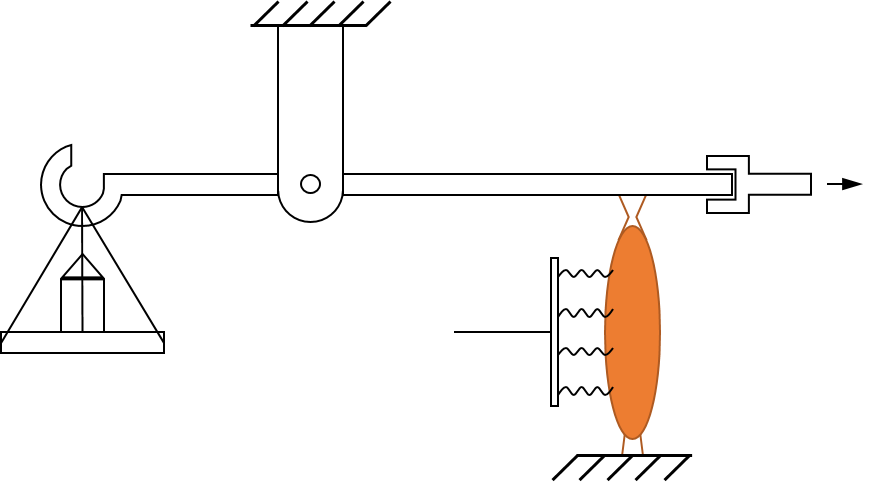
\includegraphics[width=0.9\textwidth]{misc/fig_experience_hill}};
				\node (muscle) at ($ (schema.center) + (1.45,-.7) $) {(i)};
				\node (muscle) at ($ (schema.center) + (0.55,-.45) $) {(ii)};
				\node (muscle) at ($ (schema.center) + (2.6,0.75) $) {(iii)};
				\node (muscle) at ($ (schema.center) + (-2,-1.15) $) {(iv)};
			\end{tikzpicture}
		}		
	\end{minipage}
	\begin{minipage}[b]{.4\linewidth}
		\centering
		\subcaptionbox{Hill's experimental observations\label{fig_experience_hill_1938_ii}}
		{
			\begin{tikzpicture}
			\def\varXi{0.9}%
			\def\varW{2*\pi}%
			\begin{scope}[yshift = 1.7cm]
			\begin{axis}[
				scale only axis,
				axis lines=middle,
				axis line style={->},
				width=0.7*\textwidth,
				height=0.3*\textwidth,
				xmin=0,
				xmax=10,
				ymax=1.1,
				variable=t,
				yticklabels={,,},
				xticklabels={,,},
				ytick={0.5},
				xtick={5},
				ylabel={tension},
				y label style={at={(axis description cs:-.025,.5)},rotate=90,anchor=south},
				]
				\addplot[
					color=black,
					domain=0:10,
					samples=1000
					]
					%{1 - exp(-1*\varXi*\varW*x)/(sqrt(1 - \varXi^2)) };
					{t < 5 ? 1 - exp(-2*t) : 0.5}; %
					\draw[dashed, gray] (axis cs:5, 1) -- (axis cs:10, 1);
					\draw[dashed, gray] (axis cs:0, .5) -- (axis cs:5, .5);
					\node[fill=white] (T0) at (axis cs: 2, 0.5){$T_0$};
					\node[fill=white] (T) at (axis cs: 7.4, 1){$T$};
					\node (tr) at (axis cs: 5.1, 0.2){$t_r$};
			\end{axis}
			\end{scope}
			
			\begin{scope}
			\begin{axis}[
				scale only axis,
				axis lines=middle,
				axis line style={->},
				width=0.7*\textwidth,
				height=0.3*\textwidth,
				xmin=0,
				xmax=10,
				ymin=0,
				ymax=1.2,
				variable=t,
				yticklabels={,,},
				xticklabels={,,},
				ytick={0.4, 0.6, 1},
				xtick={5},
				xlabel={time},
				x label style={at={(axis description cs:0.9,-0.1)},anchor=north},
				ylabel={length},
				y label style={at={(axis description cs:0,.5)},rotate=90,anchor=south},
				]
				\addplot[
					color=orange,
					domain=0:10,
					samples=1000,
					style={thick},
					]
					{t < 5 ? 1 : 0.2 + 1/(0.5*t)}; %
				\draw[dashed, gray] (axis cs:5, 1) -- (axis cs:10, 1);
				\draw[dashed, gray] (axis cs:3, 0.35) -- (axis cs:10, 0.35);
				\draw[dashed, gray] (axis cs:3, 0.6) -- (axis cs:10, 0.6);
				% arrows
				% delta x1
				\node (s1) at (axis cs: 7, 0.6){};
				\coordinate (d1) at (axis cs: 7, 1){};
				\draw[-{Latex[length=1.8mm]}] (s1.center) -- node[right]{\small $\Delta x_1$} (d1.center);
				\draw[-{Latex[length=1.8mm]}] (d1.center) -- (s1.center);
				% delta x2
				\node (s2a) at (axis cs: 3.5, 0.85){};
				\coordinate (d2a) at (axis cs: 3.5, 0.6){};
				\draw[-{Latex[length=1.8mm]}] (s2a.center) -- (d2a.center);
				\node (s2b) at (axis cs: 3.5, 0.15){};
				\coordinate (d2b) at (axis cs: 3.5, 0.35){};
				\draw[-{Latex[length=1.8mm]}] (s2b.center) -- node[near end, yshift=2.25mm, xshift=-1.5mm]{\small $\Delta x_2$} (d2b.center);
			\end{axis}
			\end{scope}
			\end{tikzpicture}
		}
	\end{minipage}
	}% resizebox
	\caption{ (\subref{fig_experience_hill_1938_i}) Expérience réalisée par Hill sur le gastrocnemius d'une grenouille (i), avec le stimulateur (ii) permettant de tétaniser la muscle, le mécanisme (iii) maintenant le muscle dans une configuration isométrique et la charge (iv). Ce schéma est une reproduction issue de \cite[Chapter~1]{mcmahon_muscles_1984}. (\subref{fig_experience_hill_1938_ii}) Jusqu'à $t_r$, l'expérience est dans la configuration dépeinte à gauche, la tension exercée par le muscle est $T$. Puis, le mécanisme libère la barre, le muscle se contracte alors rapidement de $\Delta x_1$, et la tension chute à une valeur de $T_0$ ce qui correspond à un comportement en raideur non amortie $K_{SEE}$, puis on observe une contraction graduelle en l'absence de changement de tension, ce qui une raideur $K_{PEE}$ amortie.}
	\label{fig_experience_hill_1938}
\end{figure}